\chapter{Dasar Teori}
\label{chap:dasar_teori}
Pada bab ini akan dijelaskan dasar-dasar teori mengenai Android SDK, Google VR SDK,Kuaternion, \textit{Sensor Fusion}, dan algoritma \textit{Head Motion Detection}.

% 2.1 Android SDK
\section{Android SDK}
\label{sec:android_sdk}

Android SDK(\textit{software development kit}) adalah kumpulan \textit{source code, development tools, emulator,}\cite{developers2011android} dan semua \textit{libraries} untuk membuat suatu aplikasi untuk \textit{platform} Android. IDE (\textit{integrated development environment} yang resmi untuk Android SDK adalah Android Studio. Android Studio dapat di download di halaman situs web Google Developer\cite{developers2011android}, sekaligus dengan Android SDKnya.  

% 2.1.1 Struktur File Android Studio Project
\subsection{Struktur File Android Studio Project}
\cite{android_developers}
		Dalam membuat aplikasi pada perangkat Android, dibutuhkan Android SDK. Android SDK(\textit{software development kit}) adalah kumpulan \textit{source code, development tools, emulator,}\cite{developers2011android} dan semua \textit{libraries} untuk membuat suatu aplikasi untuk \textit{platform} Android. IDE (\textit{integrated development environment} yang resmi untuk Android SDK adalah Android Studio. Android Studio dapat di download di halaman situs web Google Developer\cite{developers2011android}, sekaligus dengan Android SDKnya.  
				 textbf{Struktur File Android Studio Project} \\
				Pada saat \textbf{project} baru telah dibuat, Android Studio akan membuatkan folder-folder standar seperti pada Gambar \ref{fig:android-studio-structure}.
				\begin{figure}[htbp]
				\dirtree{%
					.1 {module}.
					.2 {build} \ldots{} \begin{minipage}[t]{5cm}Folder yang mengandung file-file dari hasil pembangunan \textit{project}{.}\end{minipage}.
					.2 {libs} \ldots{} \begin{minipage}[t]{5cm}Folder yang mengandung \textit{libraries} privat{.}\end{minipage}.
					.2 {src} \ldots{} \begin{minipage}[t]{5cm}Folder yang mengandung semua kode dan file sumber untuk suatu modul{.}\end{minipage}.
					.3 {androidTest} \ldots{} \begin{minipage}[t]{5cm}Folder yang mengandung kode untuk mengetes yang berjalan di perangkat Android{.}\end{minipage}.
					.3 {main} \ldots{} \begin{minipage}[t]{5cm}Folder yang mengandung file-file kode dan file sumber inti dari suatu module{.}\end{minipage}.
					.4 {AndroidManifest.xml} \ldots{} \begin{minipage}[t]{5cm}File yang mendeskripsikan sifat dari aplikasi dan setiap komponennya{.}\end{minipage}.
					.4 {java} \ldots{} \begin{minipage}[t]{5cm}Folder yang mengandung kode-kode java{.}\end{minipage}.
					.4 {jni} \ldots{} \begin{minipage}[t]{5cm}Folder yang mengandung kode-kode yang menggunakan Java Native Interface (JNI){.}\end{minipage}.
					.4 {gen} \ldots{} \begin{minipage}[t]{5cm}Folder yang mengandung file-file java yang dihasilkan oleh Android Studio{.}\end{minipage}.
					.4 {res} \ldots{} \begin{minipage}[t]{5cm}Folder yang mengandung file-file sumber untuk aplikasi, seperti file drawable, layout, dan UI String{.}\end{minipage}.
					.4 {assets} \ldots{} \begin{minipage}[t]{5cm}Folder yang mengandung file yang akan di kompile menjadi file .apk{.}\end{minipage}.
					.2 {build.gradle} \ldots{} \begin{minipage}[t]{5cm}File yang mendefinisikan konfigurasi modul untuk proses build{.}\end{minipage}.
					.1 {build.gradle} \ldots{} \begin{minipage}[t]{5cm}File yang mendefinisikan konfigurasi proses build untuk project yang berlaku untuk semua modul{.}\end{minipage}.
				}
				\caption{Tampilan struktur folder pada \textit{project} Android Studio}
				\label{fig:android-studio-structure}
				\end{figure}
				Gambar \ref{fig:android-studio-structure-screenshot} merupakan \textit{screenshot} dari project pada IDE Android Studio.
				Folder \textbf{App} pada Gambar \ref{fig:android-studio-structure-screenshot} merupakan folder \textit{module}.
				
				\begin{figure}[htbp]
					\centering
						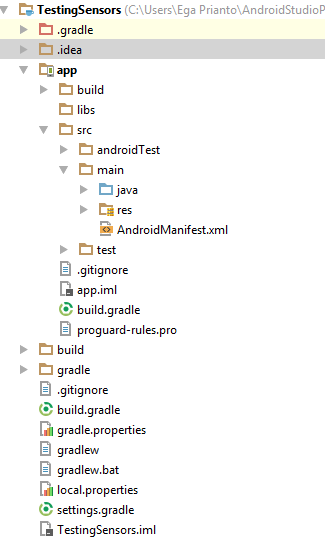
\includegraphics[scale=1]{Gambar/android-studio-structure.png}
					\caption{Tampilan struktur folder pada \textit{project} Android Studio}
					\label{fig:android-studio-structure-screenshot}
				\end{figure}

% 2.1.2 Membuat User Interface
\subsection{Membuat User Interface}
\cite{android_developers}
Pada subbab ini akan dijelaskan bagaimana membuat layout di XML termasuk \textit{text field} dan \textit{button}

% Sub 2.1.2 Hierarki (GUI) untuk Aplikasi Android
\subsubsection{Hierarki \textit{Graphical User Interface} (GUI) untuk Aplikasi Android}
\label{sssec:hierarki_gui_untuk_aplikasi_android}
GUI untuk aplikasi Android dibuat dengan hierarki dari objek View dan ViewGroup (Gambar \ref{fig:viewgroup}). Objek-objek dari View biasanya adalah \textit{UI(User Interface) Widgets} seperti \textit{button} atau \textit{text field}. Objek-objek dari ViewGroup tidak terlihat oleh \textit{view containers} yang mendefinisikan bagaimana \textit{child views} ditata seperti \textit{grid} atau \textit{vertical list}.

\begin{figure}[htbp]
	\centering
		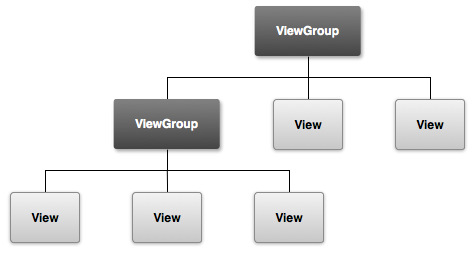
\includegraphics[scale=1]{Gambar/viewgroup.png}
	\caption{Illustrasi bagaimana percabangan objek ViewGroup pada \textit{layout} dan mengandung objek View lainnya.}
	\label{fig:viewgroup}
\end{figure}

Android menggunakan file XML yang berkorespondesi kepada \textit{subclasses} dari View dan ViewGroup, sehingga UI dapat didefinisikan dalam XML menggunakan hierarki dari elemen UI.

\subsubsection{Attribut-attribut Objek View}
\label{sssec:attribut_attribut_objek_view}
Pada subbab ini akan dijelaskan attribut-attribut object View yang digunakan dalam membuat GUI pada file activity\_main.xml
\begin{itemize}
	\item \textbf{android:id}
	Attribut ini merupakan pengidentifikasi dari suatu view. Attribut ini dapat digunakan untuk menjadi referrensi object dari kode aplikasi seperti membaca dan memanipulasi objek tersebut (Akan dijelaskan lebih lanjut pada subbab \ref{sec:activity}). Tanda '@' dibutuhkan ketika mereferensi object dari suatu XML. Tanda '@' tersebut diikuti dengan tipe (id pada kasus ini), \textit{slash}, dan nama (edit\_message pada Listing \ref{lst:attribute-view}). Tanda tambah (+) sebelum tipe hanya dibutuhkan jika ingin mendefinisikan \textit{resource ID} untuk pertama kalinya.
	\item \textbf{android:layout\_width} dan \textbf{android:layout\_height}
	Attribut ini digunakan untuk mendefinisikan panjang dan lebar dari suatu objek View. Daripada menggunakan besar spesifik untuk panjang dan lebarnya, lebih baik menggunakan "wrap\_content" yang menspesifikasi viewnya hanya akan sebesar yang dibutuhkan untuk memuat konten-konten dari View. Jika menggunakan "match\_parent" pada kasus Listing \ref{lst:attribute-view} View akan memenuhi layar, karena besarnya akan mengikuti besar dari paretnya LinearLayout.


	\item \textbf{android:hint}
	Attribut ini merupakan \textit{default string} untuk di tampilkan ketika objek View kosong. Daripada menggunakan \textit{hard-coded string} sebagai \textit{nilai} untuk ditampilkan, \textit{value} "@string/edit\_message" mereferensi ke sumber string pada file yang berbeda. Karena mereferensi ke sumber konkrit, maka tidak dibutuhkan tanda tambah (+). Nilai string ini akan di simpan pada file Strings.xml yang ditunjukkan pada Listing \ref{lst:string-xml}.
	\begin{lstlisting}[caption={Contoh kode pada string.xml},label={lst:string-xml},language=xml]
	<resources>
    <string name="app_name">MyFirstAndroidApp</string>
    <string name="edit_message">Ini adalah hint</string>
    <string name="button_send">Send</string>
	</resources>

\end{lstlisting}


	\item \textbf{android:onClick}
	Attribut ini akan memberitahu \textit{system} untuk memanggil method yang sesuai namanya (contoh pada Listing \ref{lst:attribute-view} adalah \textbf{sendMessage()}) di Activity ketika pengguna melakukan klik pada \textit{button} tersebut. Agar \textit{system} dapat memanggil method yang tepat, method tersebut harus memenuhi kriteria berikut.
	\begin{itemize}
		\item \textit{Access Modifier} haruslah \textit{public}.
		\item Harus \textit{void return value}nya.
		\item Mempunyai View sebagai parameter satu-satunya. View ini akan diisi dengan View yang di klik.
	\end{itemize}
\begin{lstlisting}[caption={Contoh kode file XML pada folder layout},label={lst:attribute-view},language=xml]
	<LinearLayout
		xmlns:android="http://schemas.android.com/apk/res/android"
		xmlns:tools="http://schemas.android.com/tools"
		android:layout_width="match_parent"
		android:layout_height="match_parent"
		android:orientation="horizontal">
		<EditText android:id="@+id/edit_message"
				android:layout_weight="1"
				android:layout_width="0dp"
				android:layout_height="wrap_content"
				android:hint="@string/edit_message" />
		<Button
				android:layout_width="wrap_content"
				android:layout_height="wrap_content"
				android:text="@string/button_send"
				android:onClick="sendMessage" />
	</LinearLayout>
\end{lstlisting}
\end{itemize}


\subsection{Activity}
\label{sec:activity}
\cite{android_developers}
Activity adalah suatu hal yang terfokuskan dengan apa yang bisa pengguna lakukan. Hampir semua \textit{Activity} berinteraksi dengan pengguna, jadi kelas Activity akan membuat suatu halaman baru yang bisa ditambahkan dengan konten-konten View. Selain dapat direpresentasikan kepada pengguna dengan halaman \textit{full-screen}, Activity juga dapat direpresentasikan dengan cara lain: seperti halaman \textit{floating} atau tertanam di Activity lain.

\subsubsection{Activity Lifecycle}
\label{sssec:activity_lifecycle}
\begin{figure}[htbp]
	\centering
		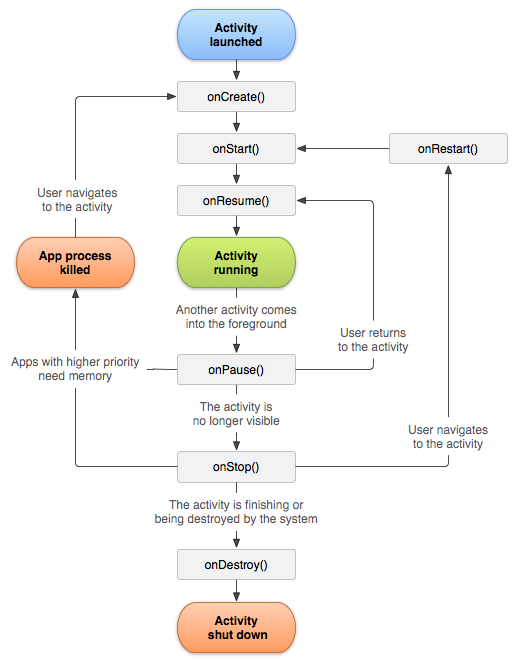
\includegraphics[scale=0.48]{Gambar/activity-lifecycle.png}
	\caption{\textit{State diagram} siklus Activity}
	\label{fig:activity-lifecycle}
\end{figure}

Aktivitas dalam sistem android di atur sebagai \textit{activity stack}. Ketika ada Activity baru yang dimulai, Activity tersebut ditempatkan di paling atas pada \textit{stack} dan menjadi Activity aktif. Activity sebelumnya akan tetap berada di bawah stack, dan tidak akan muncul lagi sampai Activity yang baru berakhir. 

Activity didasari dari empat kondisi:
\begin{itemize}
	\item Jika Activity berada di latar depan pada layar, Activity tersebut sedang aktif.
	\item Jika Activity sudah tidak terfokuskan tetapi masih dapat terlihat, Activity tersebut sedang berhenti sementara. Pada kondisi ini Activity tersebut masih berjalan, tapi bisa diberhentikan ketika system berada dalam situasi kekurangan memori.
	\item Jika suatu Activity benar-benar dihalangi oleh Activity lain, Activity tersebut telah berhenti. Activity tersebut akan tetap mengingat seluruh keadaan dan infomasi anggota tetapi, Activity tersebut tidak lagi terlihat oleh pengguna jadi tampilan jendelanya akan tersembunyi dan seringkali akan diberhentikan Activitynya ketika system membutuhkan memori.
	\item Jika suatu Activity sedang berhenti sementara atau berhenti total, sistem dapat membuang Activity dari memory dengan cara menanyakan kepada pengguna untuk memberhentikannya atau langsung diberhentikan oleh sistem. Jika Activity tersebut ditampilkan lagi kepada pengguna, Activity tersebut harus memulai dari awal dan kembali ke keadaan sebelumnya.
\end{itemize}
Gambar \ref{fig:activity-lifecycle} menunjukkan pentingnya alur keadaan dari suatu Activity. Gambar segi empat merepresentasikan \textit{callback methods} yang dapat diimplementasikan untuk melakukan operasi ketika Activity berubah kondisi. Oval berwarna merupakan kondisi-kondisi utama dari suatu Activity.
Ada 3 \textit{key loops} untuk memantau suatu Activity:
\begin{itemize}
	\item \textit{Entire lifetime} terjadi diantara pemanggilan pertama pada onCreate(Bundle) sampai ke satu pemanggilan akhir onDestroy(). Suatu Activity akan melakukan semua persiapan pada kondisi umum pada method onCreate(), dan melepaskan seluruh sisa pemrosesan pada method onDestroy().
	\item \textit{Visible lifetime} terjadi antara pemanggilan onStart() sampai pemanggilan yang sesuai pada onStop(). Pada tahap ini pengguna dapat melihat Activity pada layar meskipun tidak berada pada \textit{foreground} dan berinteraksi dengan pengguna.
	\item \textit{Foreground lifetime} terjadi antara pemanggilan method onResume() sampai ke satu pemanggilan akhir onDestroy(). Pada tahap ini Activity berada di depan semua Activity lainnya dan sedang berinteraksi dengan user.
\end{itemize}


\subsection{Android Sensor Framework}
\label{sec:android_sensor_framework}
\cite{android_developers}Sebagian besar dari perangkat android sudah memiliki sensor yang mengukur gerakan, orientasi, dan berbagai keadaan lingkungan. Sensor-sensor ini dapat memberikan data mentah dengan tingkat akurasi yang tinggi. Sensor ini juga berguna untuk memantau pergerakan tiga dimensi atau posisi perangkat. Sensor ini juga dapat memantau perubahan keadaan lingkungan yang dekat dengan perangkat. 
Android mendukung tiga kategori sensor:
\begin{itemize}
	\item \textbf{Sensor gerak}
	Sensor-sensor ini mengukur akselerasi dan rotasi pada tiga sumbu. Kategori sensor ini meliputi \textit{accelerometers}, sensor gravitasi, \textit{gyroscope}, dan \textit{rotation vector}. 
	\item \textbf{Sensor keadaan lingkungan}
	Sensor-sensor ini mengukur berbagai keadaan lingkungan seperti suhu udara, tekanan, pencahayaan, dan kelembaban. Kateori sensor ini termasuk barimeter, fotometer dan termometer.
	\item \textbf{Sensor posisi}
	Sensor-sensor ini mengukur posisi perangkat. Kategori sensor ini meliputi sensor orientasi dan magnetometer.
\end{itemize}
Android Sensor Framework membantu developers untuk mengakses berbagai jenis sensor. Beberapa sensor berbasis perangkat keras dan beberapa sensor berbasis perangkat lunak. Sensor berbasis perangkat keras mendapatkan data dengan langsung mengukur sifat lingkungan tertentu, seperti percepatan, kekuatan medan geomagnetik, atau perubahan sudut. Sensor berbasis perangkat lunak mendapatkan data dari satu atau lebih sensor berbasis perangkat keras. Sensor berbasis perangkat lunak ini juga terkadang disebut sensor virtual atau sensor sintetis. Pada tabel berikut akan dirincikan tipe-tipe setiap sensor posisi dan gerak, deskripsi, dan penggunaan umumnya.

\begin{table}[htbp]
	\centering
	\caption{Tipe-tipe Sensor pada Android}
\begin{tabular}{|p{6.3cm}| p{1.5cm}| p{5cm}| p{2.4cm}|} 
\hline
Sensor & Tipe & Deskripsi & Penggunaan umum\\ \hline
TYPE\_ACCELEROMETER & Perangkat Keras & Mengukur percepatan dalam \(m/s^2\) yang terjadi pada perangkat di semua tiga sumbu fisik (x,y,z), termasuk percepatan gravitasi. & Deteksi gerak(goncangan, keseimbangan, dan lain-lain)\\ \hline
TYPE\_GRAVITY & Perangkat Lunak atau Perangkat Keras & Mengukur percepatan gravitasi dalam \(m/s^2\) yang terjadi pada perangkat di tiga sumbu fisik (x,y, dan z) & Deteksi gerak(goncangan, keseimbangan, dan lain-lain)\\ \hline
TYPE\_GYROSCOPE & Perangkat Keras & Mengukur rata-rata rotasi sudut dalam \(rad/s\) di tiga sumbu fisik (x,y, dan z). & Deteksi rotasi (putaran, belokan, dan lain-lain).\\ \hline
TYPE\_LINEAR\_ACCELERATION & Perangkat Lunak atau Perangkat Keras & Mengukur percepatan dalam \(m/s^2\) yang terjadi pada perangkat di semua tiga sumbu fisik (x,y,z), tidak termasuk percepatan gravitasi. & Memantau percepatan pada suatu sumbu.\\ \hline
TYPE\_MAGNETIC\_FIELD & Perangkat Keras & Mengukur medan magnet sekitar untuk semua tiga sumbu fisik (x,y, dan z) di satuan \(\mu T\). & Membuat Kompas.\\ \hline
TYPE\_ORIENTATION & Perangkat Lunak & Mengukur derajat rotasi yang terjadi pada perangkat pada semua tiga sumbu fisik (x,y, dan z). & Menentukan posisi perangkat \\ \hline
TYPE\_ROTATION\_VECTOR & Perangkat Lunak dan Perangkat Keras & Mengukur orisentasi dari suatu perangkat dengan menyediakan tiga element dari vektor rotasi perangkat. & Deteksi gerak dan deteksi rotasi.\\ \hline
\end{tabular}
\end{table}
\subsubsection{Sistem Koordinat Sensor}
\label{sssec:sistem_koordinat_sensor}
Pada umumnya, sensor framework menggunakan sistem tiga sumbu koordinat standar untuk mengekspresikan nilai data. Sebagian besar sensor sistem koordinat didefinisikan relatif terhadap layar perangkat bila perangkat dibuat dalam orientasi standar (lihat Gambar \ref{fig:axis-device})
\begin{figure}[htbp]
	\centering
		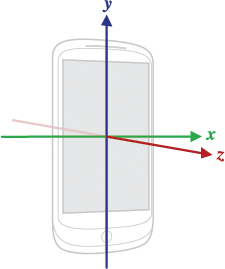
\includegraphics[scale=1]{Gambar/axis-device.png}
	\caption{Sistem koordinat (relatif dengan perangkatnya) yang digunakan oleh Sensor API}
	\label{fig:axis-device}
\end{figure}
Sensor-sensor yang menggunakan sistem tiga sumbu seperti Gambar \ref{fig:axis-device} adalah sebagai berikut :
\begin{itemize}
	\item Accelerometer
	\item Sensor Gravitasi
	\item Gyroscope
	\item Sensor Percepatan Linear
	\item Sensor Medan Geomagnetik
\end{itemize}
Koordinat sistem yang sumbunya tidak tertukar ketika orientasi perangkat berubah. Sistem koordinat sensor tidak pernah berubah seiring perangkatnya bergerak. Dalam aplikasi android tidak dapat diassumsikan bahwa standar orientasi perangkat android adalah \textit{portrait}. Kebanyakan perangkat \textit{Tablet} standar orientasinya adalah \textit{landscape}. Sistem koordinat sensor selalu di dasarkan pada orientasi dasar dari suatu perangkat android.
\subsubsection{Mengidentifikasi Sensor dan Kapabilitas Sensor}
\label{sssec:mengidentifikasi_sensor_dan_kapabilitas_sensor}
Android Sensor Framework menyediakan beberapa method yang dapat membuat developer mudah untuk menentukan sensor mana yang akan digunakan. APInya juga dapat menyediakan method yang memungkinkan penggunanya menentukan kapabilitas masing-masing sensor, seperti jangkauan maksimum, resolusi, dan kebutuhan dayanya.
Untuk mengidentifikasi sensor-sensor yang ada pada perangkat, hal pertama yang perlu dilakukan adalah mendapatkan referensi sensor tersebut. Untuk mendapatkan referensi tersebut, dapat dilakukan dengan membuat instansiasi dari kelas SensorManager dan memanggul method getSystemService() dan memasukkan isi Parameternya dengan SENSOR\_SERVICE. Contohnya pada Listing \ref{lst:init-sensor-manager}.
 
\begin{lstlisting}[caption={Contoh inisialisasi kelas SensorManager},label={lst:init-sensor-manager},language=java]
private SensorManager mSensorManager;
...
mSensorManager = (SensorManager) getSystemService(Context.SENSOR_SERVICE);
\end{lstlisting}

Kemudian untuk mendapatkan daftar dari setiap sensor pada suatu perangkat dapat dilakukan dengan cara memanggil method getSensorList() dan menggunakan konstanta TYPE\_ALL pada kelas Sensor. Contohnya pada Listing \ref{lst:get-sensor-lists}

\begin{lstlisting}[caption={Contoh untuk mendapatkan daftar dari setiap sensor yang ada},label={lst:get-sensor-lists},language=java]
List<Sensor> deviceSensors = mSensorManager.getSensorList(Sensor.TYPE_ALL);
\end{lstlisting}

Namun jika ingin mendapatkan sensor-sensor yang sesuai dengan tipe sensor yang diberikan, dapat menggunakan TYPE\_GYROSCOPE, TYPE\_LINEAR\_ACCELERATION, TYPE\_GRAVITY, atau TYPE\_GRAVITY.

Untuk menentukan jenis tertentu dari sensor yang ada pada perangkat dapat didapatkan dengan method getDefaultSensor() dengan dimasukkan dengan konstanta yang berada pada kelas Sensor. Jika perangkatnya memiliki lebih dari satu sensor dari tipe sensor yang diberikan, salah satu dari sensor tersebut akan dianggap sebagai sensor dasar. Jika sensor dasanya tidak ada untuk sensor tersebut, perangkat tersebut berarti tidak memiliki sensor dengan jenis yang diberikan. Listing \ref{lst:check-sensor} adalah contoh untuk mengecek apakah perangkat yang digunakan memiliki sensor dengan jenis yang diberikan.

\begin{lstlisting}[caption={Contoh untuk mengecek apakah perangkat yang digunakan memiliki sensor dengan jenis yang diberikan},label={lst:check-sensor},language=java]
private SensorManager mSensorManager;
...
mSensorManager = (SensorManager) getSystemService(Context.SENSOR_SERVICE);
if (mSensorManager.getDefaultSensor(Sensor.TYPE_MAGNETIC_FIELD) != null){
  // Sukses! Perangkat ini memiliki sensor magnetometer.
  }
else {
  // Gagal! Perangkat ini tidak memiliki sensor magnetometer.
  }
\end{lstlisting}

Jika ingin membatasi versi atau vendor dari sensor yang akan digunakan, dapat menggunakan method getVendor() dan getVersion(). Seperti pada Listing \ref{lst:check-sensor-version} yang mengharuskan sensor gravitasi bervendor "Google Inc." dan memiliki versi 3. Jika sensor tersebut tidak tersedia pada perangkat, sensor accelerometerlah yang digunakan.

\begin{lstlisting}[caption={Contoh untuk mengecek apakah perangkat yang digunakan memiliki sensor dengan jenis yang diberikan},label={lst:check-sensor-version},language=java]
private SensorManager mSensorManager;
private Sensor mSensor;

...

mSensorManager = (SensorManager) getSystemService(Context.SENSOR_SERVICE);
mSensor = null;

if (mSensorManager.getDefaultSensor(Sensor.TYPE_GRAVITY) != null){
  List<Sensor> gravSensors = mSensorManager.getSensorList(Sensor.TYPE_GRAVITY);
  for(int i=0; i<gravSensors.size(); i++) {
    if ((gravSensors.get(i).getVendor().contains("Google Inc.")) &&
       (gravSensors.get(i).getVersion() == 3)){
      // menggunakan sensor gravitasi versi 3.
      mSensor = gravSensors.get(i);
    }
  }
}
if (mSensor == null){
  // Use the accelerometer.
  if (mSensorManager.getDefaultSensor(Sensor.TYPE_ACCELEROMETER) != null){
    mSensor = mSensorManager.getDefaultSensor(Sensor.TYPE_ACCELEROMETER);
  }
  else{
    // Tidak ada sensor gravitasi dan sensor accelerometer!
  }
}
\end{lstlisting}

Salah satu method yang sangat berguna lagi adalah, getMinDelay(). Method ini digunakan untuk mengetahui minimum interval waktu suatu sensor dapat menerima data dalam mikrodetik. Jika method getMinDelay() mengembalikan nilai nol, hal ini berarti sensor ini akan mengembalikan data setiap kali ada perubahan nilai pada sensor tersebut. 

\subsubsection{Memonitor Nilai Sensor}
\label{sssec:memonitor_nilai_sensor}

Untuk memonitor data mentah dari sensor, dibutuhkan untuk mengimplement dua buah method callback yang berada pada interface SensorEventListener. Kedua method tersebut adalah onAccuracyChanged(Sensor sensor, int accuracy) dan onSensorChanged(SensorEvent event). Sistem android akan memanggil kedua method ini ketika terjadi salah satu kondisi ini:

\begin{itemize}
	\item \textbf{Perubahan akurasi sensor.}\\
Dalam kasus ini sistem memanggil method onAccuracyChanged(Sensor sensor, int accuracy). Parameter sensor akan diberikan objek Sensor yang telah berubah akurasinya, dan parameter accuracy adalah nilai akurasi sensor yang baru.
	\item \textbf{Sensor memberitahu adanya nilai baru.}\\
Dalam kasus ini sistem memanggil method onSensorChanged(SensorEvent event), dengan parameter event akan diisi dengan objek SensorEvent untuk mendapatkan nilai barunya. Objek SensorEvent Mengandung semua infromasi tentang data sensor yang baru, termasuk: akurasi dari data, sensor yang mendapatkan data, dan catatan waktu data tersebut didapatkan, dan data yang baru yang telah didapatkan.
\end{itemize}

Pada Listing \ref{lst:monitoring-light-sensor} akan ditunjukkan bagaimana menggunakan method onSensorChanged(SensorEvent event) untuk memonitor data dari sensor cahaya. Pada Listing \ref{lst:monitoring-light-sensor} akan menampilkan data mentah dari sensor ke TextView yang telah didefinisikan pada file main.xml sebagai sensor\_data.
\begin{lstlisting}[caption={Contoh memonitor data mentah pada sensor cahaya},label={lst:monitoring-light-sensor},language=java]
public class SensorActivity extends Activity implements SensorEventListener {
  private SensorManager mSensorManager;
  private Sensor mLight;

  @Override
  public final void onCreate(Bundle savedInstanceState) {
    super.onCreate(savedInstanceState);
    setContentView(R.layout.main);

    mSensorManager = (SensorManager) getSystemService(Context.SENSOR_SERVICE);
    mLight = mSensorManager.getDefaultSensor(Sensor.TYPE_LIGHT);
  }

  @Override
  public final void onAccuracyChanged(Sensor sensor, int accuracy) {
    // Hal yang perlu dilakukan aplikasi ketika akurasinya berubah.
  }

  @Override
  public final void onSensorChanged(SensorEvent event) {
    // Sensor cahaya akan mengembalikan 1 nilai saja.
    // Banyak sensor lain yang akan mengembalikan lebih dari 1 nilai.
    float lux = event.values[0];
    // Hal yang perlu dilakukan ketika ada perubahan data.
  }

  @Override
  protected void onResume() {
    super.onResume();
    mSensorManager.registerListener(this, mLight, SensorManager.SENSOR_DELAY_NORMAL);
  }

  @Override
  protected void onPause() {
    super.onPause();
    mSensorManager.unregisterListener(this);
  }
}
\end{lstlisting}
Pada method onSensorChanged(SensorEvent event), struktur nilai-nilai yang dikembalikan akan dijelaskan pada subbab \ref{sssec:struktur_nilai_yang_dikembalikan_oleh_sensor}. Pada method onResume(), ada pemanggilan method registerListener(). Method registerListener() ini berguna untuk menspesifikasikan waktu delay pada pemanggilan onSensorChanged(). Untuk menspesifikasikan delaynya dapat menggunakan konstanta yang ada pada kelas SensorManager. Konstanta-konstanta tersebut adalah SENSOR\_DELAY\_NORMAL (200.000 mikrodetik),SENSOR\_DELAY\_GAME (20.000 mikrodetik),SENSOR\_DELAY\_UI (60.000 mikrodetik), atau SENSOR\_DELAY\_FASTEST (0 mikrodetik). Pengaturan dasar untuk waktu delay ini menggunakan konstanta SENSOR\_DELAY\_NORMAL.
Perlu diperhatikan juga pemesanan sensor ketika activity sedang di berhentikan sementara maupun dilanjutkan kembali. Sistem tidak boleh tetap merekam sensor ketika activity tidak aktif. Hal ini diperlukan karena pada saat perangkat android menggunakan sensor, perangkat akan menggunakan tenanga yang banyak. Akan lebih baik jika penggunaan sensor diberhentikan ketika activitynya sudah tidak lagi digunakan. 
\subsubsection{Struktur Nilai yang Dikembalikan oleh Sensor}
\label{sssec:struktur_nilai_yang_dikembalikan_oleh_sensor}
Setiap sensor android akan mengembalikan nilai-nilainya dengan struktur-struktur tertentu. Pada bab ini akan dijelaskan secara detil struktur nilai sistem android dalam mengembalikan nilai-nilai yang diperoleh dari sensor. Nilai ini akan didapatkan dengan tipe data array of float. Besar dan isi dari array tergantung pada sensor yang sedang di pantau. Berikut ini adalah struktur-struktur nilai dari setiap sensor pada sistem android :\\
\begin{itemize}
	\item \textbf{TYPE\_ACCELEROMETER}\\
Semua nilai didefinisikan sebagai satuan \(m/s^2\)
\begin{itemize}
	\item values[0]: Percepatan yang terjadi pada sumbu x dikali -1
	\item values[1]: Percepatan yang terjadi pada sumbu y dikali -1
	\item values[2]: Percepatan yang terjadi pada sumbu z dikali -1
\end{itemize}
Sensor ini mengukur percepatan(\(Ad\)) yang diterapkan pada perangkat. Sensor tersebut dapat mengukur percepatan dengan mengukur gaya(\(Fs\)) yang terjadi pada sensor menggunakan relasi berikut:
\[
	Ad = -\Sigma Fs / mass
\]
Secara khusus, gravitasi selalu mempengaruhi percepatan yang diukur :
\[
	Ad =  -g -\Sigma F / mass
\]
Karena inilah ketika perangkat android sedang diam, accelerometer membaca percepatan gravitasi sebesar \(g = 9.81m/s^2\).
Demikian pula ketika perangkat android sedang dalam keadaan jatuh bebas. Perangkat akan mempercepat menuju ke tanah pada percepatan \(9.81 m/s^2\), sehingga accelerometer membaca percepatan total sebesar \( 0 m/s^2\). 
Suatu saat akan di butuhkan untuk mengukur percepatan asli yang terjadi pada perangkat, sehingga kontribusi gravitasi harus di eliminasi. Hal ini bisa dilakukan dengan menerapkan \textit{high-pass} filter. Sebaliknya, \textit{low-pass} filter dapat digunakan untuk mendapatkan nilai gravitasi saja. 
\begin{lstlisting}[caption={Implementasi \textit{low-pass} filter},label={lst:low-pass-filter},language=java]
	 public void onSensorChanged(SensorEvent event)
     {
          // alpha dikalkulasikan sebagai t / (t + dT)
          // dengan t adalah low-pass filter's time-constant
          // dan dT, rata-rata event tersampaikan

          final float alpha = 0.8;

          gravity[0] = alpha * gravity[0] + (1 - alpha) * event.values[0];
          gravity[1] = alpha * gravity[1] + (1 - alpha) * event.values[1];
          gravity[2] = alpha * gravity[2] + (1 - alpha) * event.values[2];

          linear_acceleration[0] = event.values[0] - gravity[0];
          linear_acceleration[1] = event.values[1] - gravity[1];
          linear_acceleration[2] = event.values[2] - gravity[2];
     }
\end{lstlisting}
\textit{Low-pass} filter dapat diimplementasikan pada Listing \ref{lst:low-pass-filter}\\
\item \textbf{TYPE\_MAGNETIC\_FIELD}\\
Sensor ini mengukur medan magnet sekitar perangkat pada sumbu X,Y, dan Z dalam satuan micro-Tesla.\\
\item \textbf{TYPE\_GYROSCOPE}\\
Sensor ini mengukur rata-rata perputaran pada perangkat yang berputar di sumbu X,Y, dan Z dalam satuan radians/second. Sistem koordinat yang digunakan sama dengan sistem koordinat pada sensor percepatan(Accelerometer). Jika perangkat berputar berlawanan arah jarum jam pada sumbu tertentu, maka rotasi yang terjadi akan bernilai positif. Perhatikan bahwa standar perputaran ini adalah definisi matematika standar pada rotasi positif.
\begin{itemize}
	\item values[0]: Percepatan angular pada sumbu X.
	\item values[1]: Percepatan angular pada sumbu Y.
	\item values[2]: Percepatan angular pada sumbu Z.
\end{itemize}
Biasanya keluaran dari gyroscope terintegrasi dari waktu ke waktu untuk menghitung rotasi yang menggambarkan perubahan sudut atas langkah waktu, misalnya pada Listing \ref{lst:gryoscope-example}
\begin{lstlisting}[caption=contoh implementasi gyroscope,label={lst:gryoscope-example},language=java]
	  private static final float NS2S = 1.0f / 1000000000.0f;
     private final float[] deltaRotationVector = new float[4]();
     private float timestamp;

     public void onSensorChanged(SensorEvent event) {
          // Pada tahapan ini delta rotasi akan dikalikan dengan rotasi saat ini
          // setelah mengomputasinya dari data gyro.
          if (timestamp != 0) {
              final float dT = (event.timestamp - timestamp) * NS2S;
              // Sumbu dari rotasi, masih belum di normalisasi.
              float axisX = event.values[0];
              float axisY = event.values[1];
              float axisZ = event.values[2];

              // Menghitung percepatan angular
              float omegaMagnitude = sqrt(axisX*axisX + axisY*axisY + axisZ*axisZ);

              // Normalisasi rotasi vektor jika cukup besar untuk mendapatkan sumbunya.
              if (omegaMagnitude > EPSILON) {
                  axisX /= omegaMagnitude;
                  axisY /= omegaMagnitude;
                  axisZ /= omegaMagnitude;
              }

              // Integrate around this axis with the angular speed by the time step
              // in order to get a delta rotation from this sample over the time step
              // We will convert this axis-angle representation of the delta rotation
              // into a kuaternion before turning it into the rotation matrix.
              float thetaOverTwo = omegaMagnitude * dT / 2.0f;
              float sinThetaOverTwo = sin(thetaOverTwo);
              float cosThetaOverTwo = cos(thetaOverTwo);
              deltaRotationVector[0] = sinThetaOverTwo * axisX;
              deltaRotationVector[1] = sinThetaOverTwo * axisY;
              deltaRotationVector[2] = sinThetaOverTwo * axisZ;
              deltaRotationVector[3] = cosThetaOverTwo;
          }
          timestamp = event.timestamp;
          float[] deltaRotationMatrix = new float[9];
          SensorManager.getRotationMatrixFromVector(deltaRotationMatrix, deltaRotationVector);
          // User code should concatenate the delta rotation we computed with the current rotation
          // in order to get the updated rotation.
          // rotationCurrent = rotationCurrent * deltaRotationMatrix;
     }
     }
\end{lstlisting}
Dalam prakteknya, gyroscope \textit{noise} dan \textit{offset} akan menyebabkan beberapa kesalahan yang harus dikompensasi. Cara untuk mengkompensasinya biasanya dilakukan dengan menggunakan informasi dari sensor lain.\\
\item \textbf{TYPE\_GRAVITY}\\
Sensor ini menunjukkan arah dan besarnya vektor gaya gravitasi. Sensor ini mengembalikan nilai dengan satuan \(m/s^2\). Sistem koordinat sama seperti sistem koordinat yang umum digunakan sensor percepatan. 

Catatan: Bila perangkat sedang diam, maka keluaran dari sensor gravitasi harus identik dengan accelerometer. \\

\item \textbf{TYPE\_LINEAR\_ACCELERATION}\\
Sensor yang menunjukkan percepatan pada setiap sumbu perangkat, tidak termasuk percepatan yang terjadi karena gravitasi. Nilai diberikan dalam satuan \(m/s^2\). Sistem koordinat yang digunakan sama seperti sistem koordinat yang digunakan sensor percepatan. Keluaran dari sensor accelerometer, gravitasi dan percepatan linear harus mengikuti aturan berikut:
\[
	percepatan = gravitasi + percepatan linear
\]\\

\item \textbf{TYPE\_ORIENTATION}\\
Semua nilai adalah sudut dalam derajat.
\begin{itemize}
	\item values[0]: Azimuth, sudut diantara arah magnetik utara dengan sumbu y, sekitar sumbu z (0 sampai 359). 0 = Utara, 90 = Timur, 180 = Selatan, 270 = Barat
	\item values[1]: Pitch, rotasi sekitar sumbu x (-180 sampai 180), dengan nilai positif ketika sumbu x bergerak menuju sumbu y.
	\item values[2]: Roll, perputaran sekitar sumbu y (-90 sampai 90) pada kondisi potrait, sensor akan bernilai 0. Pada kondisi landscape ke kanan sensor akan bernilai 90 dan sebaliknya yaitu kondisi landscape ke kiri sensor akan bernilai -90.
\end{itemize}

Catatan: Definisi ini berbeda dengan definisi yaw, pitch, dan roll yang digunakan pada aviasi yang sumbu X adalah sepanjang sisi bidang.

Catatan: Sensor ini sudah tidak digunakan lagi(deprecated), yang digunakan sekarang adalah sensor rotasi vector.\\
\item \textbf{TYPE\_ROTATION\_VECTOR}\\
Sensor ini merepresentasikan orientasi perangkat dengan kombinasi dari sumbu dan sudut. Perangkat akan di putar sebesar sudut \(\theta\) mengelilingi sumbu \(x,y,z\). Tiga elemen dari vektor rotasi adalah (\(x \sin (\frac{\theta}{2}), y \sin (\frac{\theta}{2}), z \sin (\frac{\theta}{2})\)), sehingga besarnya vektor rotasi sama dengan \(\sin (\frac{\theta}{2})\), dan arah vektor rotasi sama dengan sumbu rotasi. Tiga elemen dari vektor rotasi sama dengan tiga komponen terakhir pada unit kuaternion(\(\cos (\frac{\theta}{2}),x \sin (\frac{\theta}{2}), y \sin (\frac{\theta}{2}), z \sin (\frac{\theta}{2})\)) yang dijelaskan pada subbab \ref{sec:teori_quaternion}. Elemen dari vektor rotasi tak memiliki satuan. Sistem koordinat yang digunakan sama dengan sistem koordinat yang digunakan pada sensor percepatan. Referensi koordinat didefinisikan sebagai basis orthonormal, yaitu:
\begin{itemize}
	\item X didefinisikan sebagai perkalian dot product \textbf{Y.Z}
	\item Y merupakan tangensial ke tanan pada lokasi perangkat saat ini dan menunjuk ke arah utara. 
	\item Z menghadap ke langit dan tegak lurus dengan tanah. Untuk lebih jelasnya dapat dilihat pada Gambar \ref{fig:axis-globe}
	\begin{figure}[htbp]
	\centering
	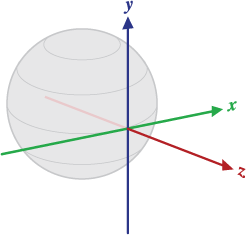
\includegraphics[scale=1]{Gambar/axis-globe.png}
	\caption{Sistem koordinat sensor rotasi vektor terhadap Bumi} 
	\label{fig:axis-globe}
	\end{figure}
	\item values[0]: \(x \sin (\frac{\theta}{2})\)
	\item values[1]: \(y \sin (\frac{\theta}{2})\)
	\item values[2]: \(z \sin (\frac{\theta}{2})\)
	\item values[3]: \(\cos (\frac{\theta}{2})\)
	\item values[4]: Perkiraan akurasi (dalam radians) (-1 jika tidak tersedia) 
\end{itemize}



\end{itemize}



\section{Google VR SDK}
\label{sec:google_vr_sdk}
Google VR SDK\cite{google_vr_developers} digunakan untuk membantu dalam pembuatan aplikasi Virtual Reality pada \textit{smartphone}. Google VR SDK memberikan beberapa fitur sebagai berikut :
\begin{itemize}
	\item \textbf{Binocular rendering}: Fitur untuk tampilan layar terpisah untuk masing-masing dalam pandangan VR.
	\item \textbf{Spatial audio}: Fitur untuk mengeluarkan suara yang datang dari daerah-daerah tertentu dari dunia VR.
	\item \textbf{Head movement tracking}: Fitur untuk mendapatkan memperbaharui pengelihatan dunia VR yang sesuai dengan gerakan kepala pengguna.
	\item \textbf{Trigger input}: Fitur untuk memberikan input pada dunia VR dengan menekan tombol.
\end{itemize}

Ada beberapa persyaratan untuk menggunakan Google VR SDK, persyaratan tersebut adalah:
\begin{itemize}
	\item Android Studio versi 1.0 atau lebih.
	\item Android SDK versi 23
	\item Gradle versi 23.0.1 atau lebih. Android Studio akan membantu meningkatkan versinya jika versinya terlalu rendah.
	\item Perangkat Android fisik yang menjalankan Android versi 4.4 (KitKat) atau lebih.
\end{itemize}

Dalam membuat aplikasi Google Cardboard VR membutuhkan beberapa API(Application Program Interface) dari Google VR SDK. API-API umum yang akan digunakan adalah sebagai berikut. 
\begin{itemize}
	\item API audio: API untuk mengimplementasikan \textbf{\textit{Spatial Audio}} (Metode untuk menspasialisasikan sumber suara dalam ruang tiga dimensi).
	\item API base: API untuk fondasi dari suatu aplikasi Google VR.
\end{itemize}

\subsection{API Audio}
\label{sec:api_audio}
\cite{google_vr_developers}
API ini membantu developer untuk menspasialisasikan sumber suara dalam tiga dimensi, termasuk jarak dengan tinggi isyarat sumber suara. Pada API ini hanya terdapat satu class utama yaitu \textbf{GvrAudioEngine}. \textbf{GvrAudioEngine} mampu memutarkan suara secara spasial dalam dua cara yang berbeda :
\begin{itemize}
	\item Metode pertama dikenal sebagai \textit{Sound Object rendering}. Metode ini memungkinkan pengguna membuat sumber suara virtual dalam ruang tiga dimensi.
	\item Metode kedua memungkinkan pengguna untuk memutar kembali rekaman \textit{Ambisonic soundfield}. Rekaman \textit{Ambisonic soundfield} adalah file audio \textit{multi-channel} yang telah terspasialisasi.
\end{itemize}
API ini juga dapat memutarkan suara secara \textit{stereo}. Kelas \textbf{GvrAudioEngine} memiliki tiga buah \textit{nested class} yaitu:
\begin{itemize}
	\item GvrAudioEngine.DistanceRolloffModel: Kelas ini mendefinisikan konstanta-konstanta yang merepresentasikan perbedaan jarak dari efek model-model rolloff. 
	\item GvrAudioEngine.MaterialName: Kelas ini mendefinisikan konstanta-konstanta yang merepresentasikan bahan permukaan ruangan untuk disesuaikan dengan efek suara pada suatu ruangan.
	\item GvrAudioEngine.RenderingMode: Kelas ini mendefinisikan konstanta-konstanta untuk menyesuaikan dengan mode rendering. Semakin baik kualitas renderin akan semakin besar penggunaan CPU(Central Processing Unit).
\end{itemize}

\subsection{API Base}
\label{sec:api_base}
\cite{google_vr_developers}
API ini digunakan sebagai fondasi dari suatu aplikasi Google VR. Fitur-fitur Binocular rendering, Head movement tracking, dan Trigger input diimplementasikan pada API ini. Kelas-kelas penting yang ada di API ini adalah AndroidCompat, Eye, GvrActivity, GvrView, HeadTransform, Viewport.
\begin{itemize}
	\item AndroidCompat\\
Kelas ini merupakan kelas utilitas untuk menggunakan fitur VR. Fitur-fitur ini mungkin tidak tersedia pada semua versi android. Kelas ini memiliki method-method sebagai berikut:
\begin{itemize}
	\item setSustainedPerformanceMode(Activity activity, boolean enabled): \\
	Method ini digunakan untuk mengubah window android ke mode performa secara berkelanjutan.
	\item public static void setVrModeEnabled (Activity activity, boolean enabled): \\
	Mengatur pengaturan yang tepat untuk "mode VR" pada suatu Activity. Method ini tidak digunakan karena hanya dapat digunakan pada Android N+.
	\item public static boolean trySetVrModeEnabled (Activity activity, boolean enabled): 
	Method ini kegunaanya sama dengan method \textbf{setVrModeEnabled (Activity activity, boolean enabled)}, namun mengembalikan boolean true jika berhasil dan sebaliknya.
\end{itemize}
	\item Eye\\
Kelas ini mendefinisikan detil perenderan stereoskopik mata. Method penting yang dimiliki kelas ini adalah \textbf{public float[] getEyeView ()}. Method ini mengembalikan matriks yang mentransformasikan camera virtual ke mata. Transformasi yang diberikan termasuk melacak rotasi kepala, perubahan posisi dan perubahan IPD(interpupillary distance).
	\item GvrActivity\\
Kelas ini merupakan Activity dasar yang menyediakan integrasi yang mudah dengan headset Google VR. Kelas ini mengekspos kejadian untuk berinteraksi dengan headset Google VR dan menangani detil-detil yang biasa diperlukan saat membuat suatu Activity untuk perenderan VR. Activity ini membuat layar tetap menyala selama perangkat android bergerak. Jika tidak ada pergerakan dari perangkat android maka layar reguler (\textit{wakeclock}) akan ditampilkan. Pada kelas ini terdapat method \textbf{onCardboardTrigger ()} untuk mendeteksi ketika Cardboard Trigger sedang ditarik dan dilepaskan (Magnet yang berada pada sisi Google Cardboard).
	\item GvrView\\
	Kelas ini merupakan kelas View yang menyediakan perenderan VR. Kelas ini didesain untuk berkerja pada mode layar penuh dengan orientasi \textit{landscape} atau \textit{reverse landscape}. Kelas View ini dapat digunakan dengan mengimplements salah satu Interface perenderan. Interface-interface tersebut adalah:
	\begin{itemize}
		\item GvrView.StereoRenderer: Interface untuk perenderan detil stereoskopik secara abstrak oleh perender.
		\item GvrView.Renderer: Interface untuk mesin yang kompleks yang membutuhkan untuk menangai semua detil perenderan.
	\end{itemize}
Kelas GvrView.Renderer jarang digunakan dan sebaiknya tidak digunakan jika tidak sangat dibutuhkan.
Ketika suatu kelas mengimplement Kelas GvrView.StereoRenderer, kelas tersebut harus mengimplementasikan method-method berikut ini:
\begin{itemize}
	\item \textbf{public void onNewFrame(HeadTransform headTransform)}\\
	method ini terpanggil ketika Framebaru akan digambar. Method ini memungkinkan untuk membedakan antara perenderan pandangan mata dan frame-frame yang berbeda. Setiap operasi per-frame harus tidak spesifik pada satu tampilan saja.
	\item \textbf{public abstract void onDrawEye (Eye eye)}\\
	Method ini meminta untuk menggambar suatu konten dari sudut pandang mata.
	\item \textbf{public abstract void onFinishFrame (Viewport viewport)}\\
	Method ini dipanggil ketika suatu frame telah selesai. Dengan pemanggilan ini, konten frame telah di gambar dan jika koreksi distorsi diaktifkan, koreksi distrosi akan diterapkan. Setiap perendereran pada tahap ini relatif terhadap seluruh permukana, tidak terhadap satu pandangan mata tunggal. 
	\item \textbf{public abstract void onRendererShutdown ()}\\
	Method ini dipanggil ketika thread perender sedang menutup. Melepaskan sumber GL(Graphics Library) dan sedang melakukan penutupan operasi pada thread perender. Dipanggil hanya jika sebelumnya ada pemanggilan method onSurfaceCreated.
	\item \textbf{public abstract void onSurfaceChanged (int width, int height)}\\
	Dipanggil ketika ada perubahan dimensi permukaan. Semua nilai adalah relatif ke ukuran yang dibutuhkan untuk merender sebuah mata.
	\item \textbf{public abstract void onSurfaceCreated (EGLConfig config)}\\
	Method ini dipanggil ketika suatu permukaan dibangun atau dibangun ulang.
\end{itemize}
\item HeadTransform\\
	Method ini mendeskripsikan transformasi kepala secara independen dari setiap parameter mata. Kelas ini digunakan di kelas GvrView.StereoRenderer sebagai parameter pada method \textbf{onNewFrame}. Method-method yang perlu diperhatikan pada kelas ini adalah:
	\begin{itemize}
		\item \textbf{public void getHeadView (float[] headView, int offset)}\\
		Method ini digunakan untuk mendapatkan matriks transformasi dari camera virtual ke kepala. Kepala disini didefinisikan sebagai titik tengah diantara kedua mata. Matriks yang didapatkan akan disimpan pada parameter \textbf{headView}.
		\item \textbf{public void getQuaternion (float[] quaternion, int offset)}\\
		Method ini digunakan untuk mendapatkan kuaternion yang merepresentasikan rotasi kepala.
	\end{itemize}
	\item Viewport\\
	Kelas ini didefinisikan sebagai \textit{viewport}(area pandang) berbentuk persegi.
\end{itemize}
\section{Teori Kuaternion}
\label{sec:teori_quaternion}

Pada Android SDK \textbf{SensorEvent.values} \cite{android_developers} tipe sensor \textbf{Sensor.TYPE\_ROTATION\_VECTOR}, yaitu tipe sensor yang mendeteksi vektor perputaran pada \textit{smartphone}. Tipe sensor ini dijelaskan akan mengembalikan nilai-nilai dari komponen kuaternion. 
Kuaternion\cite{kuipers:1999} adalah objek penggabungan dari suatu skalar dengan suatu vektor, sesuatu yang tidak dapat didefinisikan dalam aljabar linear biasa. Kuaternion ditemukan oleh William Rowan Hamilton dengan memperpanjang notasi dari bilangan kompleks menjadi Kuaternion. 
\subsection{Struktur Ajabar}
Karena Kuaternion merupakan bilangan kompleks yang diperpanjang notasinya, struktur aljabar Kuaternion hampir mirip dengan bilangan kompleks. Untuk mengerti struktur-struktur aljabar kuaternion, diperlukan untuk mengerti  bilangan kompleks terlebih dahulu. Berikut adalah penjelasan singkat tentang bilangan kompleks. 


\subsubsection{Bilangan Kompleks}
\label{sssec:bilangan_kompleks}
\cite{kuipers:1999}
Bilangan kompleks adalah bilangan yang merupakan gabungan dari bilangan imajiner dengan bilangan riil. Notasi umum dari bilangan kompleks adalah :

\begin{equation}
	a+bi
\label{eq:notasi_umum_bilangan_kompleks}
\end{equation}
Pada notasi \ref{eq:notasi_umum_bilangan_kompleks} bilangan \(a\) dengan \(b\) merupakan bilangan riil, dan \(i\) merupakan bilangan imajiner tertentu yang memiliki sifat \(i^2=-1\). Bilangan kompleks juga dapat beroperasi dengan bilangan kompleks lainnya seperti penjumlahan, perkalian, pengurangan, dan pembagian. Berikut adalah contoh-contoh operasi pada bilangan kompleks \ref{eq:notasi_umum_bilangan_kompleks} dengan bilangan kompleks \(c+di\):
\begin{itemize}
	\item Penjumlahan\\
	\[
	 (a + bi) + (c + di) = (a+c) + i(b+d)
	\]
	\item Perkalian\\
	\[
	 (a + bi)(c + di) = (ac−bd) + (bc+ad)i
	\]
	\item Pengurangan\\
	\[
	 (a + bi) - (c + di) = (a-c) + i(b-d)
	\]
	\item Pembagian\\
	\[
	 \frac{(a + bi)}{(c + di)} = \frac{(ac+bd)}{c^2+d^2} + i \frac{bc-ad}{c^2+d^2}
	\]
\end{itemize}
Pada operasi penjumlahan dan perkalian untuk kedua bilangan kompleks tersebut memiliki hukum assosiatif dan komutatif. Notasi \ref{eq:penjumlahan_hukum} menunjukkan bagaimana bagaimana kedua hukum tersebut berlaku pada penjumlahan.
\begin{equation}
	\begin{split}
	(a+ib) + (c+id) = (a+c) + i(b+d)=\\
	(c+id) + (a+ib) = (c+a) + i(d+b)
	\end{split}
\label{eq:penjumlahan_hukum}
\end{equation}

Suatu bilangan dapat dikatakan konjugasi kompleks dari suatu bilangan kompleks jika nilai bilangan riilnya sama, tetapi nilai bilangan imajinernya berlawanan dengan nilai pada bilangan kompleks tersebut. Maka konjugasi kompleks dari bilangan kompleks \ref{eq:notasi_umum_bilangan_kompleks} adalah \(a-bi\). 

Bilangan kompleks ini dapat digunakan untuk rotasi vektor pada bidang dua dimensi. Rotasi ini dapat dilakukan dengan mengalikan suatu vektor dengan bilangan imajiner $i$. Mengalikan suatu vektor dengan bilangan imajiner $i$ akan memutar vektor sebesar $90^{\circ}$ berlawanan arah jarum jam. Mengalikan suatu vektor dengan bilangan imajiner $i^2$ akan memutar vektor sebesar $180^{\circ}$ berlawanan arah jarum jam. Untuk memperjelas perputaran dengan bilangan kompleks diberikan contoh berikut:
Sebuah vektor $v = 3 + i3$ akan diputar $90^{\circ}$ berlawanan arah jarum jam dengan mengalikan vektor tersebut dengan bilangan imajiner $i$. Maka vektor hasil perputarannya($v'$) adalah :
\begin{equation}
	\begin{split}
		v' = &i(3 + i3)\\
		= & i3 + i^2 3\\
		= & i3 + (-1) 3\\
		= & -3 + i3
	\end{split}
\label{eq:rotasi_kompleks}
\end{equation}
\begin{figure}[htbp]
\centering
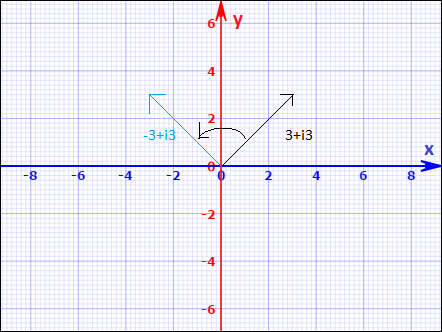
\includegraphics[scale=1]{Gambar/diagram-rotasi-kompleks.png}
\caption{Contoh perputaran dengan bilangan kompleks} 
\label{fig:diagram-rotasi-kompleks}
\end{figure}
Dengan bilangan pada bilangan riil diasumsikan sebagai nilai pada sumbu x dan bilangan yang dikalikan dengan bilangan $i$ diasumsikan pada sumbu y($x + iy$) Seperti yang ditunjukkan pada Gambar \ref{fig:diagram-rotasi-kompleks}. Oleh karena itu rumus perputaran menggunakan bilangan kompleks dapat di rumuskan sebagai berikut: 
\[
	v' = v\times(\cos \theta + i \sin \theta)
\]
dengan $\theta$ adalah besar sudut perputaran. Jika vektor $v = 3 + i3$ diputar $30^{\circ}$ berlawanan arah jarum jam menggunakan konsep diatas, akan menghasilkan vektor berikut:

\begin{equation}
	\begin{split}
		v' = &(3 + i3)(\cos 30^{\circ} + i \sin 30^{\circ})\\
		= & (3 + i3)(\frac{\sqrt{3}}{2} + i \frac{1}{2})\\
		= & \frac{3\sqrt{3}-3}{2} + i\frac{3\sqrt{3}+3}{2}\\
		= & 1.098 + i4.098
	\end{split}
\label{eq:rotasi_kompleks_tiga_puluh_derajat}
\end{equation}

Dari persamaan tersebut dapat divisualisasikan pada Gambar \ref{fig:diagram-rotasi-kompleks1}.

\begin{figure}[htbp]
\centering
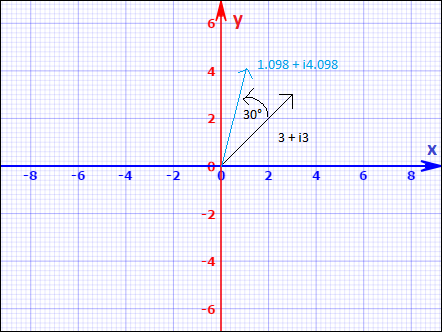
\includegraphics[scale=1]{Gambar/diagram-rotasi-kompleks1.png}
\caption{Contoh perputaran tiga puluh derajat dengan bilangan kompleks} 
\label{fig:diagram-rotasi-kompleks1}
\end{figure}
\subsection{\textit{Aljabar Kuaternion} dan Operasi-operasi pada Kuaternion}
\cite{kuipers:1999}
Kuaternion ditemukan oleh ahli matematika dan astronomi Inggris, William Rowan Hamilton, dengan memperpanjang aritmatika dari bilangan kompleks. Dari penemuan tersebut William Rowan Hamilton menemukan bahwa dia tidak hanya membutuhkan bilangan imajiner \(i\) saja untuk melakukan rotasi pada ruang tiga dimensi. Dia menemukan bahwa dia juga membutuhkan tiga komponen imajiner lainnya yaitu \(i,j\) dan \(k\). Persamaan umum Kuaternion memiliki empat bilangan riil atau skalar. Persamaan tersebut adalah 

\begin{equation}
	q = q_0 + i q_1 + j q_2 + k q_3	
\label{eq:notasi_kuaternion}
\end{equation}
Ketiga komponen tersebut memiliki relasi sebagai berikut:
\[
	i^2 = j^2 = k^2 = ijk = -1
\]

Hasil dari perkalian dua \textit{kuaternion} memiliki aturan yang lebih rumit, sehingga memiliki aturan-aturan khusus. Berikut aturan-aturan khususnya :
\begin{equation}
	\begin{split}
	& ij = k = -ji\\
	& jk = i = -kj\\
	& ki = j = -ik	
	\end{split}
\label{eq:persamaan_khusus_aturan_quaternion}
\end{equation}\\
Ketiga persamaan diatas mirip dengan aturan tangan kanan (\textit{right-hand rule})pada perkalian cross product dari suatu vector. Pada Gambar \ref{fig:right-hand-rule}, \(A\) berperan sebagai \(i\), \(B\) berperan sebagai \(j\), dan \(C\) berperan sebagai \(k\).\\
\begin{figure}[htbp]
\centering
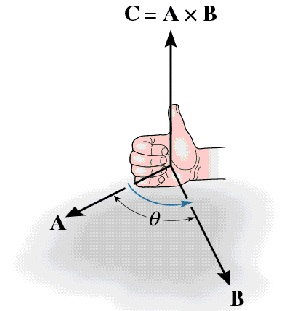
\includegraphics[scale=1]{Gambar/right-hand-rule}
\caption{Right-hand rule dalam \textit{cross product} vektor} 
\label{fig:right-hand-rule}
\end{figure}\\

Seperti pada bilangan kompleks, kuaternion juga memiliki konjugasinya. Konjugasi kuaternion ini akan digunakan untuk melakukan operasi rotasi tiga dimensi(Akan dijelaskan pada subsubbab berikut). Sama dengan konjugasi pada bilangan kompleks, kuaternion yang bilangan riilnya sama, dan bilangan imajinernya berlawanan dengan kuaternionnya disebut dengan konjugasi kuaternion. Oleh karena itu konjugasi kuaternion dari notasi kuaternion \ref{eq:notasi_kuaternion} adalah: 
\[
	q = q_0 - i q_1 - j q_2 - k q_3
\]
\subsubsection{Operasi pada Kuaternion}
\label{sssec:operasi_pada_kuaternion}
Dua buah kuaternion dapat dikatakan identik jika dan hanya jika kedua kuaternion memiliki komponen yang identik.
\[
	p = p_0 + +ip_1+jp_2+kp_3
\]
dan,
\[
	q = q_0 + i q_1 + j q_2 + k q_3
\]
maka p = q jika dan hanya jika
\begin{equation}
	\begin{split}
	p_0=q_0\\
	p_1=q_1\\
	p_2=q_2\\
	p_3=q_3\\
	\end{split}
\end{equation}
Penjumlahan dari kedua kuaternion diatas dapat didefinisikan sebagai komponen penjumlahan yaitu:
\[
	(p+q)=(p_0+q_0)+i(p_1+q_1)+j(p_2+q_2)+k(p_3+q_3)
\]
Perkalian dari kedua kuaternion diatas dapat didefinisikan sebagai komponen perkalian yaitu:
\[
	pq = (p_0 +ip_1+jp_2+kp_3)(q_0 + i q_1 + j q_2 + k q_3)
\]
Begitu pula untuk komponen pengurangan dengan pembagian. 
Dari keempat operasi kuaternion tersebut, operasi kuaternion yang digunakan untuk rotasi bidang tiga dimensi adalah operasi perkalian. Fungsi rotasi vektor dapat menggunakan operasi kuaternion seperti pada bilangan kompleks, dengan rumus:
\[
	v' = qvq^*
\]
dengan,
\begin{itemize}
	\item \(v = 1 + x_v i +y_v j + z_v k\)
	\item \(q = q_0 + i q_1 + j q_2 + k q_3	\)
	\item \(q^* =  q_0 - i q_1 - j q_2 - k q_3\)
	\item \(v' = 1 + x_{v'} i +y_{v'} j + z_{v'} k\)
\end{itemize}
Seperti pada bilangan kompleks, bilangan $q_0 ,i q_1,j q_2,k q_3$ akan memiliki nilai sebagai berikut jika suatu kuaternion ingin digunakan untuk rotasi tiga dimensi:
\begin{equation}
	\begin{split}
	q_0=& \cos (\frac{\theta}{2})\\
	q_1=& \sin (\frac{\theta}{2}) x_f\\
	q_2=& \sin (\frac{\theta}{2}) y_f\\
	q_3=& \sin (\frac{\theta}{2}) z_f\\
	\end{split}
\end{equation}
dengan vektor f ($x_f,y_f,z_f$) merupakan sumbu perputaran dan $\theta$ merupakan besar sudut putar berlawanan arah dengan jarum jam.